\documentclass{beamer}

\usepackage{graphics}
\usepackage{graphicx}
\usepackage{amsmath,amssymb,amsthm}
%\usepackage{subeqnarray}
%\usepackage{easybmat}
%\usepackage{subfigure}



%\usepackage{HA-prosper}
%\usepackage[dvips,letterpaper]{geometry}

\def\Proba#1{\mathcal{P}\left(#1\right)}
\def\Surv{\mathcal{S}}
\def\R{\mathcal{R}}
\def\D{\mathcal{D}}
\def\C{\mathcal{C}}
\def\M{\mathcal{M}}
\def\L{\mathcal{L}}
\def\IC{\mathbb{C}}
\def\IN{\mathbb{N}}
\def\IR{\mathbb{R}}
\def\IZ{\mathbb{Z}}
\def\IK{\mathbb{K}}
\def\II{\mathbb{I}}
\def\Rzero{\mathcal{R}_0}
\newcommand{\diag}{\operatorname{diag}}
\def\tr{\textrm{tr}}
\def\det{\textrm{det}}
\def\sgn{\textrm{sgn}}
\def\imply{$\Rightarrow$}
\def\dbint{\int\!\!\!\int}
\def\dbintb{\mathop{\int\!\!\!\!\int}}
\def\tpint{\int\!\!\!\int\!\!\!\int}

\def\red{\color[rgb]{1,0,0}}

\newtheorem{proposition}{Proposition}

\setbeamertemplate{navigation symbols}{}
\setbeamertemplate{footline}
{%
\quad\insertsection\hfill p. \insertpagenumber\quad\mbox{}\vskip2pt
}

\title[Traffic flow]{Traffic flow\\[1.5cm] Linear cascades\\ Linear systems\\
Delay differential equations\\ Laplace transform}
\date{}

\begin{document}
\frame[plain]{\setcounter{page}{0}\titlepage}
%%%%%%%%%%%%%%
%%%%%%%%%%%%%%


\section{Traffic flow -- ODE model}
\frame[plain]{\tableofcontents[current]}


\frame{\frametitle{Problem formulation}
Want to model
\begin{itemize}
\item $N$ cars
\item on a straight road
\item no overtaking
\item adjustment of speed on driver in front
\end{itemize}
}

\frame{\frametitle{Hypotheses}
\begin{itemize}
\item $N$ cars in total.
\item Road is the $x$-axis.
\item $x_n(t)$ position of the $n$th car at time $t$.
\item $v_n(t)\stackrel{\Delta}{=}x_n'(t)$ velocity of the $n$th car at time $t$.
\end{itemize}
\begin{center}
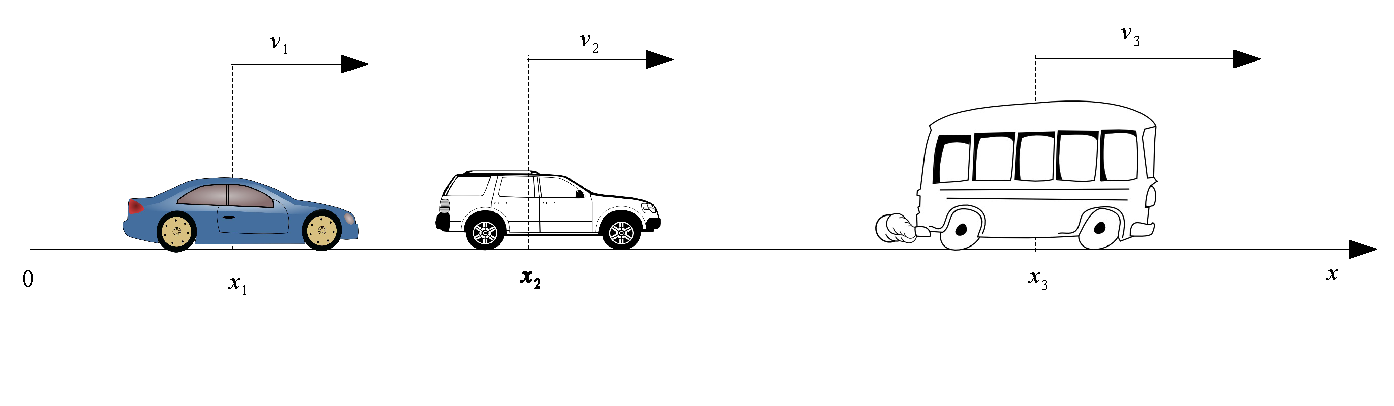
\includegraphics[width=\textwidth]{traffic_flow1}
\end{center}
\begin{itemize}
\item All cars start with the same initial speed $v_0$ before time $t=0$.
\end{itemize}
}

\frame{\frametitle{Moving frame coordinates}
To make computations easier, express velocity of cars in a reference frame moving at speed $u_0$.
\vskip1cm
Remark that here, speed=velocity, since movement is 1-dimensional.
\vskip1cm
Let
\[
u_n(t)=v_n(t)-u_0.
\]
Then $u_n(t)=0$ for $t\leq 0$, and $u_n$ is the speed of the $n$th car in the moving frame coordinates.
}

\frame{\frametitle{Modeling driver behavior}
Assume that
\begin{itemize}
\item Driver adjusts his/her speed according to relative speed between his/her car and the car in front.
\item This adjustment is a linear term, equal to $\lambda$ for all drivers.
\end{itemize}
\vskip1cm
\begin{itemize}
\item
First car: evolution of speed remains to be determined.
\item 
Second car:
\[
u_2'=\lambda(u_1-u_2).
\]
\item
Third car:
\[
u_3'=\lambda(u_2-u_3)
\]
\item 
Thus, for $n=1,\ldots,N-1$,
\begin{equation}\label{eq:ode}
u_{n+1}'=\lambda(u_n-u_{n+1}).
\end{equation}
\end{itemize}
}


\frame{
This can be solved using \emph{linear cascades}: if $u_1(t)$ is known, then
\[
u_2'=\lambda(u_1(t)-u_2)
\]
is a linear first-order nonhomogeneous equation. Solution (integrating factors, or variation of constants) is
\[
u_2(t)=\lambda e^{-\lambda t}\int_0^t u_1(s)e^{\lambda s}ds
\]
Then use this function $u_2(t)$ in $u_3'$ to get $u_3(t)$,
\begin{align*}
u_3(t) &= \lambda e^{-\lambda t}\int_0^t u_2(s)e^{\lambda s}ds
\end{align*}
}

\frame{
Thus
\begin{align*}
u_3(t) &= \lambda e^{-\lambda t}\int_0^t u_2(s)e^{\lambda s}ds \\
&= \lambda e^{-\lambda t}\int_0^t 
\left(\lambda e^{-\lambda s}\int_0^s u_1(q)e^{\lambda q}dq\right)ds \\
&= \lambda^3 e^{-\lambda t}\int_0^t e^{-\lambda s}\int_0^s u_1(q)e^{\lambda q}dqds
\end{align*}
Continue the process to get the solution.
}

\frame{\frametitle{Example}
Suppose driver of car 1 follows this function
\[
u_1(t)=\alpha\sin(\omega t)
\]
that is, $\omega$-periodic, 0 at $t=0$ (we want all cars to start with speed relative to the moving reference equal to 0), and with amplitude $\alpha$.

\vskip0.5cm
Then
\begin{align*}
u_2(t) &= \lambda\alpha e^{-\lambda t}\int_0^t \sin(\omega s)e^{\lambda s}ds \\
&= \lambda\alpha e^{-\lambda t}
\left(
\frac{\omega-\omega e^{\lambda t} \cos(\omega t)+\lambda e^{\lambda t} \sin(\omega t)}{\lambda^2+\omega^2}
\right) \\
&= \frac{\lambda\alpha}{\lambda^2+\omega^2}\left(\omega e^{-\lambda t}
+\lambda\sin(\omega t)-\omega\cos(\omega t)\right).
\end{align*}
When $t\to\infty$, first term goes to 0, we are left with a $\omega$-periodic
term.
}


\frame{
Continuing the process,
\begin{multline*}
u_3(t) = \frac{\lambda^2\alpha}{\lambda^2+\omega^2} e^{-\lambda t}\times\\
\int_0^t \left(\omega e^{-\lambda s}
+\lambda\sin(\omega s)-\omega\cos(\omega s)\right)e^{\lambda s}ds
\end{multline*}
that is,
\begin{align*}
u_3(t) &= \frac{\lambda^2\alpha}{\lambda^2+\omega^2}e^{-\lambda t}\left(\omega t+\int_0^t \left(\lambda\sin(\omega s)-\omega\cos(\omega s)\right)e^{\lambda s}ds\right) \\
&= \frac{\lambda^2\alpha}{\lambda^2+\omega^2}\left(\omega t+\frac{2 \lambda \omega}{\lambda^2+\omega^2}\right)e^{-\lambda t}\\
&\quad -\frac{\lambda^2\alpha}{(\lambda^2+\omega^2)^2}\left(2 \lambda \omega \cos(\omega t)-\lambda^2 \sin(\omega t)+\omega^2 \sin(\omega t)\right)
\end{align*}
Once again, the terms in $e^{-\lambda t}$ vanishes for large $t$, and we are left with 3 $\omega$-periodic terms.
}

\section{Linear systems of ODE -- Brief theory}
\frame[plain]{\tableofcontents[current]}


\frame{\frametitle{Linear ODEs}
\begin{definition}[Linear ODE]
A \emph{linear} ODE is a differential equation taking the form
\begin{equation}\label{sys:linear_general}
\frac{d}{dt}x=A(t)x+B(t),\tag{LNH}
\end{equation}
where $A(t)\in\mathcal{M}_n(\IR)$ with continuous entries, $B(t)\in\IR^n$ with real valued, continuous coefficients, and $x\in\IR^n$. The associated IVP takes the form 
\begin{equation}\label{sys:IVP_linear_general}
\begin{aligned}
\frac{d}{dt}x &= A(t)x+B(t) \\
x(t_0)&=x_0.
\end{aligned}
\end{equation}
\end{definition}
}

\frame{\frametitle{Types of systems}
\begin{itemize}
\item $x'=A(t)x+B(t)$ is linear nonautonomous ($A(t)$ depends on $t$) nonhomogeneous (also called \emph{affine} system).
\item $x'=A(t)x$ is linear nonautonomous homogeneous.
\item $x'=Ax+B$, that is, $A(t)\equiv A$ and $B(t)\equiv B$, is linear autonomous nonhomogeneous (or affine autonomous).
\item $x'=Ax$ is linear autonomous homogeneous.
\end{itemize}
\vskip1cm
\begin{itemize}
\item If $A(t+T)=A(t)$ for some $T>0$ and all $t$, then linear periodic.
\end{itemize}
}


\frame{\frametitle{Existence and uniqueness of solutions}
\begin{theorem}[Existence and Uniqueness]
Solutions to \eqref{sys:IVP_linear_general} exist and are unique on the whole interval over which $A$ and $B$ are continuous.

In particular, if $A,B$ are constant, then solutions exist on $\IR$.
\end{theorem}
}

\frame{\frametitle{Autonomous linear systems}
Consider the autonomous affine system
\begin{equation}\label{sys:affine_auton}
\frac{d}{dt}x=Ax+B,\tag{A}
\end{equation}
and the associated homogeneous autonomous system
\begin{equation}\label{sys:lin_auton}
\frac{d}{dt}x=Ax.\tag{L}
\end{equation}
}

\frame{\frametitle{Exponential of a matrix}
\begin{definition}[Matrix exponential]
Let $A\in\M_n(\IK)$ with $\IK=\IR$ or $\IC$. The \emph{exponential} of $A$, denoted $e^{At}$, is a matrix in $\M_n(\IK)$, defined by
\[
e^{At}=\II +\sum_{k=1}^\infty \frac{t^k}{k!}A^k,
\]
where $\II$ is the identity matrix in $\M_n(\IK)$.
\end{definition}
}

\frame{\frametitle{Properties of the matrix exponential}
\begin{itemize}
\item $e^{At_1}e^{At_2}=e^{A(t_1+t_2)}$ for all $t_1,t_2\in\IR$.
1\item $Ae^{At}=e^{At}A$ for all $t\in\IR$.
\item $(e^{At})^{-1}=e^{-At}$ for all $t\in\IR$.
\item The unique solution $\phi$ of \eqref{sys:lin_auton} with $\phi(t_0)=x_0$ is given by
\[
\phi(t)=e^{A(t-t_0)}x_0.
\]
\end{itemize}
}

\frame{\frametitle{Computing the matrix exponential}
Let $P$ be a nonsingular matrix in $\M_n(\IR)$. We transform the IVP
\begin{equation}\label{IVP:lin_auton}
\begin{aligned}
\frac{d}{dt}x &= Ax\\
x(t_0)&=x_0
\end{aligned}\tag{L\_IVP}
\end{equation}
using the transformation $x=Py$ or $y=P^{-1}x$.
\vskip0.5cm
The dynamics of $y$ is
\begin{align*}
y' &= (P^{-1}x)' \\
&= P^{-1}x' \\
&= P^{-1}Ax \\
&= P^{-1}APy
\end{align*}
The initial condition is $y_0=P^{-1}x_0$.
}

\frame{
We have thus transformed IVP \eqref{IVP:lin_auton} into
\begin{equation}\label{IVP:lin_auton2}
\begin{aligned}
\frac{d}{dt}y &= P^{-1}APy\\
y(t_0)&=P^{-1}x_0
\end{aligned}\tag{L\_IVP\_y}
\end{equation}
From the earlier result, we then know that the solution of \eqref{IVP:lin_auton2} is given by
\[
\psi(t)=e^{P^{-1}AP(t-t_0)}P^{-1}x_0,
\]
and since $x=Py$, the solution to \eqref{IVP:lin_auton} is given by
\[
\phi(t)=Pe^{P^{-1}AP(t-t_0)}P^{-1}x_0.
\]
So everything depends on $P^{-1}AP$.
}

\frame{\frametitle{Diagonalizable case}
Assume $P$ nonsingular in $\M_n(\IR)$ such that
\[
P^{-1}AP=
\begin{pmatrix}
\lambda_1 & & 0 \\
& \ddots & \\
0 & & \lambda_n
\end{pmatrix}
\]
with all eigenvalues $\lambda_1,\ldots,\lambda_n$ different.
}


\frame{
We have
\[
e^{P^{-1}AP}=\II+\sum_{k=1}^\infty\frac{t^k}{k!}
\begin{pmatrix}
\lambda_1 & & 0 \\
& \ddots & \\
0 & & \lambda_n
\end{pmatrix}^k
\]
}

\frame{
For a (block) diagonal matrix $M$ of the form
\[
M=
\begin{pmatrix}
m_{11} & & 0\\
& \ddots & \\
0 & & m_{nn}
\end{pmatrix}
\]
there holds
\[
M^k=
\begin{pmatrix}
m_{11}^k & & 0\\
& \ddots & \\
0 & & m_{nn}^k
\end{pmatrix}
\]
}

\frame{
Therefore,
\begin{align*}
e^{P^{-1}AP} &= \II+\sum_{k=1}^\infty\frac{t^k}{k!}
\begin{pmatrix}
\lambda_1^k & & 0 \\
& \ddots & \\
0 & & \lambda_n^k
\end{pmatrix} \\
&=\begin{pmatrix}
\sum_{k=0}^\infty\frac{t^k}{k!}\lambda_1^k & & 0 \\
& \ddots & \\
0 & & \sum_{k=0}^\infty\frac{t^k}{k!}\lambda_n^k
\end{pmatrix}\\
&=\begin{pmatrix}
e^{\lambda_1t} & & 0 \\
& \ddots & \\
0 & & e^{\lambda_nt}
\end{pmatrix}
\end{align*}
}

\frame{
And so the solution to \eqref{IVP:lin_auton} is given by
\[
\phi(t)=P
\begin{pmatrix}
e^{\lambda_1t} & & 0 \\
& \ddots & \\
0 & & e^{\lambda_nt}
\end{pmatrix}
P^{-1}x_0.
\]
}


\frame{\frametitle{Nondiagonalizable case}
The Jordan canonical form is
\[
P^{-1}AP=
\begin{pmatrix}
J_0 & & 0\\
& \ddots & \\
0 & & J_s
\end{pmatrix}
\]
so we use the same property as before (but with block matrices now), and
\[
e^{P^{-1}APt}=
\begin{pmatrix}
e^{J_0t} & & 0\\
& \ddots & \\
0 & & e^{J_st}
\end{pmatrix}
\]
}

\frame{
The first block in the Jordan canonical form takes the form
\[
J_0=
\begin{pmatrix}
\lambda_0 & & 0\\
& \ddots & \\
0 & & \lambda_k
\end{pmatrix}
\]
and thus, as before,
\[
e^{J_0t}=
\begin{pmatrix}
e^{\lambda_0t} & & 0\\
& \ddots & \\
0 & & e^{\lambda_kt}
\end{pmatrix}
\]
}

\frame{
Other blocks $J_i$ are written as
\[
J_i=\lambda_{k+i}\II+N_i
\]
with $\II$ the $n_i\times n_i$ identity and $N_i$ the $n_i\times n_i$ nilpotent matrix
\[
N_i=\begin{pmatrix}
0 & 1 & 0 && 0 \\
&&\ddots && \\
&&&& 1 \\
0& &&&0
\end{pmatrix}
\]
$\lambda_{k+i}\II$ and $N_i$ commute, and thus
\[
e^{J_it}=e^{\lambda_{k+i}t}e^{N_it}
\]
}

\frame{
Since $N_i$ is nilpotent, $N_i^k=0$ for all $k\geq n_i$, and the series $e^{N_it}$ terminates, and
\[
e^{J_it}=e^{\lambda_{k+i}t}
\begin{pmatrix}
1 & t & \cdots & \frac{t^{n_i-1}}{(n_i-1)!} \\
0 & 1 & \cdots & \frac{t^{n_i-2}}{(n_i-2)!} \\
&&& \\
0 &&& 1
\end{pmatrix}
\]
}

\frame{
\begin{theorem}
For all $(t_0,x_0)\in\IR\times\IR^n$, there is a unique solution $x(t)$ to \eqref{IVP:lin_auton} defined for all $t\in\IR$. Each coordinate function of $x(t)$ is a linear combination of functions of the form
\[
t^ke^{\alpha t}\cos(\beta t)\quad\textrm{and}\quad t^ke^{\alpha t}\sin(\beta t)
\]
where $\alpha+i\beta$ is an eigenvalue of $A$ and $k$ is less than the algebraic multiplicity of the eigenvalue.
\end{theorem}
}

\frame{\frametitle{Generalized eigenvectors}
\begin{definition}[Generalized eigenvectors]
Let $A\in\M_r(\IR)$. Suppose $\lambda$ is an eigenvalue of $A$ with multiplicity $m\leq n$. Then, for $k=1,\ldots,m$, any nonzero solution $v$ of
\[
(A-\lambda\II)^kv=0
\]
is called a \emph{generalized eigenvector} of $A$.
\end{definition}
}

\frame{\frametitle{Nilpotent matrix}
\begin{definition}[Nilpotent matrix]
Let $A\in\M_n(\IR)$. $A$ is \emph{nilpotent} (of order $k$) if $A^{j}\neq 0$ for $j=1,\ldots,k-1$, and $A^k=0$.
\end{definition}
}

\frame{\frametitle{Jordan normal form}
\begin{theorem}[Jordan normal form]
Let $A\in\M_n(\IR)$ have eigenvalues $\lambda_1,\ldots,\lambda_n$, repeated according to their multiplicities. 
\begin{itemize}
\item 
Then there exists a basis of generalized eigenvectors for $\IR^n$. 
\item 
And if $\{v_1,\ldots,v_n\}$ is any basis of generalized eigenvectors for $\IR^n$, then the matrix $P=[v_1\cdots v_n]$ is invertible, and $A$ can be written as
\[
A=S+N,
\]
where
\[
P^{-1}SP=\diag(\lambda_j),
\]
the matrix $N=A-S$ is nilpotent of order $k\leq n$, and $S$ and $N$ commute, i.e., $SN=NS$.
\end{itemize}
\end{theorem}
}

\frame{
\begin{theorem}
Under conditions of the Jordan normal form Theorem, the linear system $x'=Ax$ with initial condition $x(0)=x_0$, has solution
\[
x(t)=P\diag\left(e^{\lambda_j t}\right)P^{-1}\left(\II+Nt+\cdots\frac{t^k}{k!}N^k\right) x_0.
\]
\end{theorem}
The result is particularly easy to apply in the following case.
\begin{theorem}[Case of an eigenvalue of multiplicity $n$]
Suppose that $\lambda$ is an eigenvalue of multiplicity $n$ of $A\in\M_n(\IR)$. Then $S=\diag(\lambda)$, and the solution of $x'=Ax$ with initial value $x_0$ is given by
\[
x(t)=e^{\lambda t}\left(\II+Nt+\cdots\frac{t^k}{k!}N^k\right) x_0.
\]
\end{theorem}
In the simplified case, we do not need the matrix $P$ (the basis of generalized eigenvectors).
}

\frame{\frametitle{A variation of constants formula}
\begin{theorem}[Variation of constants formula]
Consider the IVP
\begin{subequations}\label{sys:lin_nonlin}
\begin{align}
x' &= Ax+B(t) \\
x(t_0) &= x_0,
\end{align}
\end{subequations}
where $B:\IR\to\IR^n$ a smooth function on $\IR$, and let $e^{A(t-t_0)}$ be matrix exponential associated to the homogeneous system $x'=Ax$. Then the solution $\phi$ of \eqref{sys:lin_nonlin} is given by
\begin{equation}
\phi(t)=e^{A(t-t_0)}x_0 + \int_{t_0}^t e^{A(t-s)}B(s)ds.
\end{equation}
\end{theorem}
}




\section{Linear systems -- Our case}
\frame[plain]{\tableofcontents[current]}

\frame{\frametitle{Computation in our case}
Consider the case of 3 cars. Let
\[
X=\begin{pmatrix}
u_2\\ u_3
\end{pmatrix}
\]
Then the system can be written as
\[
X'=\begin{pmatrix}
-\lambda & 0 \\
\lambda & -\lambda
\end{pmatrix}U
+\begin{pmatrix}
\lambda u_1(t)\\ 0
\end{pmatrix}
\]
which we write for short as $X'=AX+B(t)$.
}

\frame[containsverbatim]{
The matrix $A$ has the eigenvalue $-\lambda$ with multiplicity 2. Its Jordan form is obtained by using the maple function {\tt JordanForm}:
\begin{verbatim}
> with(LinearAlgebra)
> A := <<-lambda, lambda> | <0, -lambda>>:
> J := JordanForm(A)
\end{verbatim}
giving
\[
J=\begin{pmatrix}
-\lambda & 1 \\
0 & -\lambda
\end{pmatrix}
\]
To get the matrix of change of basis, 
\begin{verbatim}
> P := JordanForm(A,output='Q')
\end{verbatim}
giving
\[
P=\begin{pmatrix}
0 & 1 \\
\lambda & 0
\end{pmatrix}
\]
which is such that $P^{-1}AP=J$.
}

\frame{
Because $-\lambda$ is an eigenvalue with multiplicity 2 (same as the size of the matrix), we can use the simplified theorem, and only need $N$. 
\vskip1cm
We have
\begin{align*}
N &= A-S \\
&=\begin{pmatrix}
-\lambda & 0 \\
\lambda & -\lambda
\end{pmatrix}
-
\begin{pmatrix}
-\lambda & 0 \\
0 & -\lambda
\end{pmatrix} \\
&=\begin{pmatrix}
0 & 0 \\
\lambda & 0
\end{pmatrix}
\end{align*}
}


\frame{
Clearly, $N^2=0$, so, by the theorem in the simplified case,
\begin{align*}
x(t) &= e^{-\lambda t}\left(\II+Nt\right)x_0 \\
\end{align*}
But we know that solutions are unique, and that the solution to the differential equation is given by $x(t)=e^{At}x_0$. This means that
\begin{align*}
e^{At} &= e^{-\lambda t}\left(\II+Nt\right)\\
&= e^{-\lambda t}\left(\begin{pmatrix}1&0\\0&1\end{pmatrix}+
\begin{pmatrix}
0 & 0 \\
\lambda t & 0
\end{pmatrix}\right)\\
&= e^{-\lambda t}\begin{pmatrix}
1 & 0 \\
\lambda t & 1
\end{pmatrix} \\
&= \begin{pmatrix}
e^{-\lambda t} & 0 \\
\lambda te^{-\lambda t} & e^{-\lambda t}
\end{pmatrix}
\end{align*}
}

\frame{Now notice that the solution to
\[
X'=AX
\]
is trivially established here, since
\[
X(0)=\begin{pmatrix}u_2(0)\\u_3(0)\end{pmatrix}=\begin{pmatrix}0\\0\end{pmatrix},
\]
and thus
\[
X(t)=e^{At}0=0.
\]
$e^{At}$ does however play a role in the solution (fortunately), since it is involved in the variation of constants formula:
\[
X(t)=e^{At}X_0+\int_0^t e^{A(t-s)}B(s)ds
\]
}

\frame{
Thus we need to compute $e^{A(t-s)}B(s)$, and then the integral.
\begin{align*}
e^{A(t-s)}B(s) &= 
\begin{pmatrix}
e^{-\lambda (t-s)} & 0 \\
\lambda (t-s)e^{-\lambda (t-s)} & e^{-\lambda (t-s)}
\end{pmatrix}
\begin{pmatrix}
\lambda u_1(s)\\ 0
\end{pmatrix} \\
&= \begin{pmatrix}
\lambda e^{-\lambda(t-s)}u_1(s) \\
\lambda^2e^{-\lambda(t-s)} (t-s)u_1(s)
\end{pmatrix}
\end{align*}
}

\frame{
and thus
\begin{align*}
\int_0^t e^{A(t-s)}B(s)ds &=
\int_0^t\left(
\begin{array}{ll}
\lambda e^{-\lambda(t-s)}u_1(s) \\
\lambda^2e^{-\lambda(t-s)} (t-s)u_1(s)
\end{array}
\right)ds \\
&= \left(\begin{array}{ll}
\int_0^t\lambda e^{-\lambda(t-s)}u_1(s) ds \\
\int_0^t\lambda^2e^{-\lambda(t-s)} (t-s)u_1(s) ds
\end{array}
\right) \\
&= \left(\begin{array}{ll}
\lambda e^{-\lambda t} \int_0^te^{\lambda s}u_1(s) ds \\
\lambda^2 e^{-\lambda t}\int_0^te^{\lambda s} (t-s)u_1(s) ds
\end{array}
\right) \\
&= \left(\begin{array}{ll}
\lambda e^{-\lambda t} \int_0^te^{\lambda s}u_1(s) ds \\
\lambda^2 e^{-\lambda t}\left(t\int_0^te^{\lambda s}u_1(s) ds
-\int_0^tse^{\lambda s} u_1(s) ds\right)
\end{array}
\right)
\end{align*}
}


\frame{
Let
\[
\Psi(t)=\int_0^t e^{\lambda s} u_1(s)ds
\]
and
\[
\Phi(t)=\int_0^t se^{\lambda s} u_1(s)ds
\]
These can be computed when we choose a function $u_1(t)$. Then, finally, we have
\begin{align*}
X(t) &= \int_0^t e^{A(t-s)}B(s)ds \\
&= \left(\begin{array}{ll}
\lambda e^{-\lambda t} \Psi(t) \\
\lambda^2 e^{-\lambda t}\left(t\Psi(t)
-\Phi(t)\right)
\end{array}
\right)
\end{align*}
}


\frame{\frametitle{Case of the $\alpha\sin(\omega t)$ driver}
We set
\[
u_1(t)=\alpha\sin(\omega t).
\]
Then
\begin{align*}
\Psi(t) &= \frac{\alpha (\omega-\omega e^{\lambda t} \cos(\omega t)+\lambda e^{\lambda t} \sin(\omega t))}{\lambda^2+\omega^2}
\end{align*}
and
\begin{align*}
\Phi(t) &=\frac{\alpha(\lambda^3 t+\lambda t \omega^2-\lambda^2+\omega^2) \sin(\omega t) e^{\lambda t}}{(\lambda^2+\omega^2)^2}\\
&\quad -\frac{\alpha\omega \cos(\omega t) (t \lambda^2+t \omega^2-2 \lambda) e^{\lambda t}+2\alpha \lambda \omega}{(\lambda^2+\omega^2)^2}
\end{align*}
}

\frame{
\begin{center}
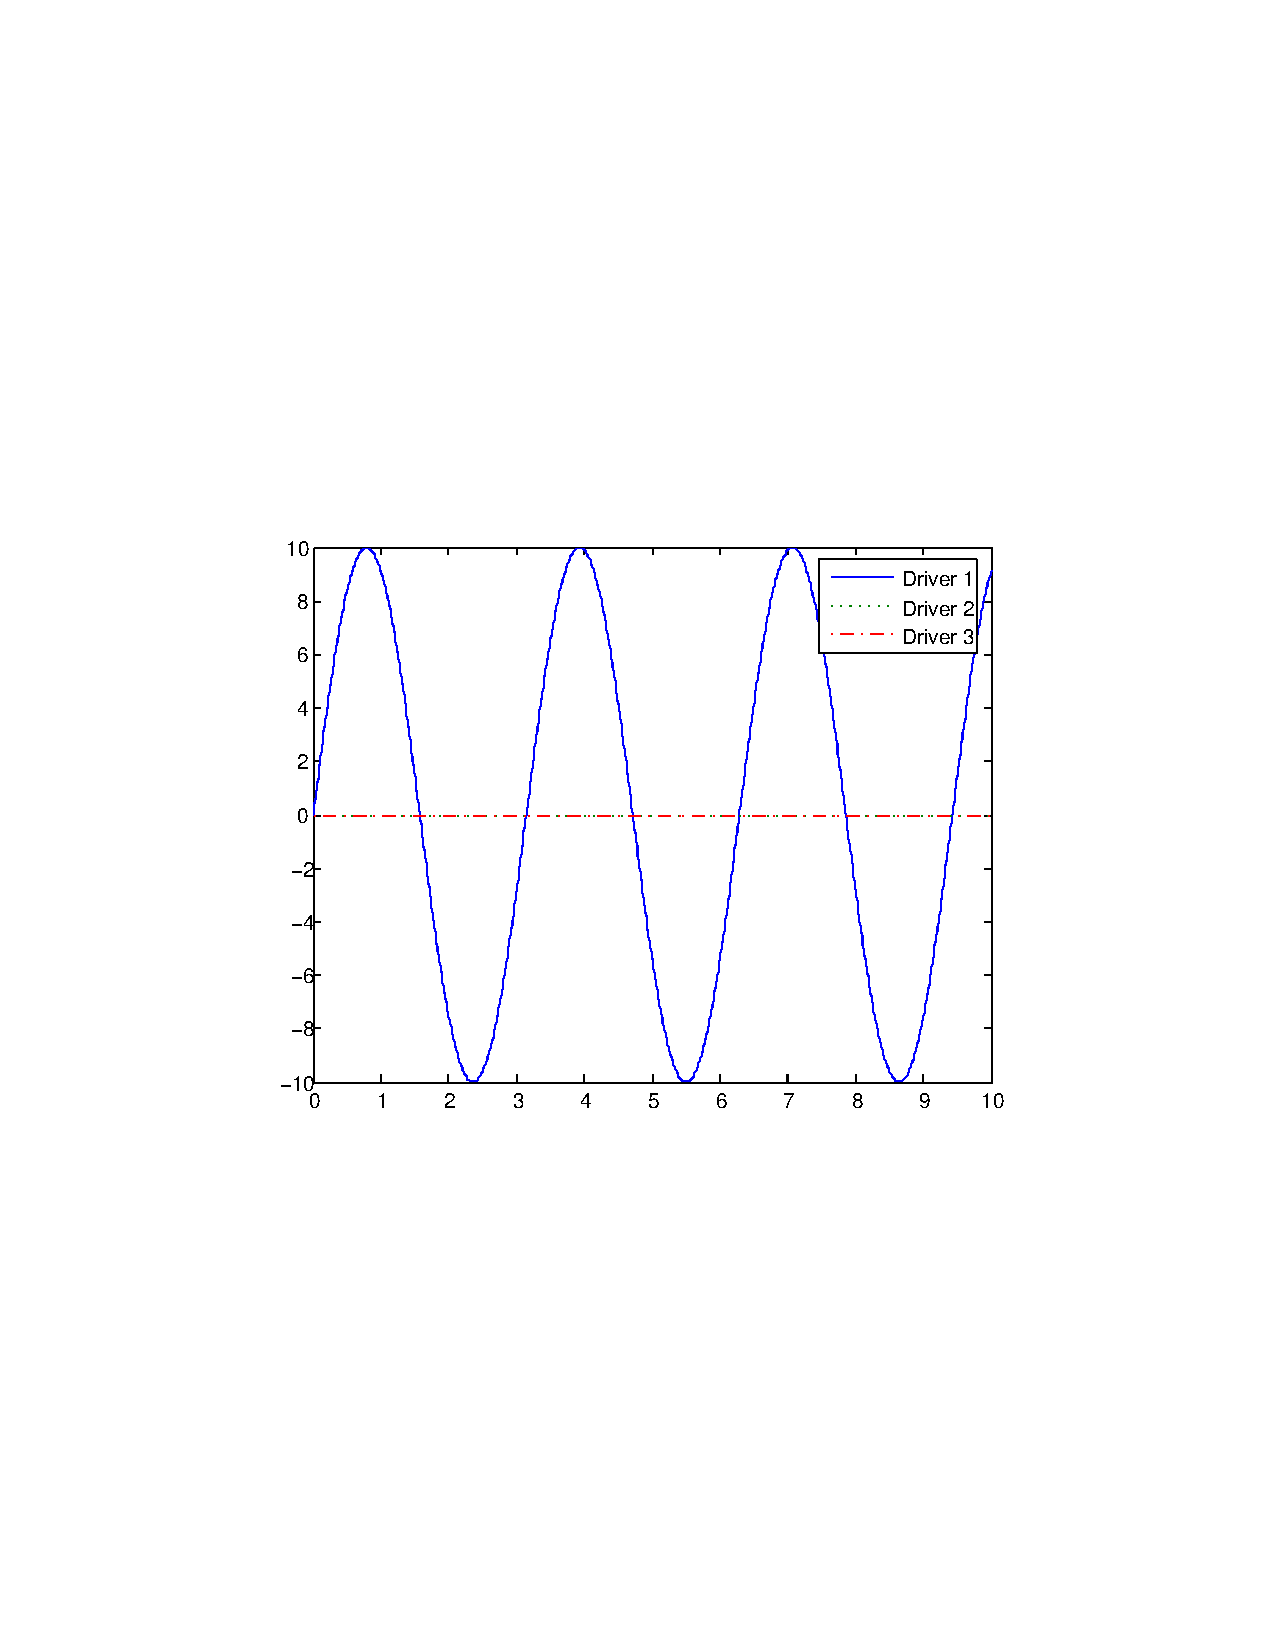
\includegraphics[width=\textwidth]{traffic_flow_3cars_ODE_l0}
\end{center}
$\lambda=0$
}
\frame{
\begin{center}
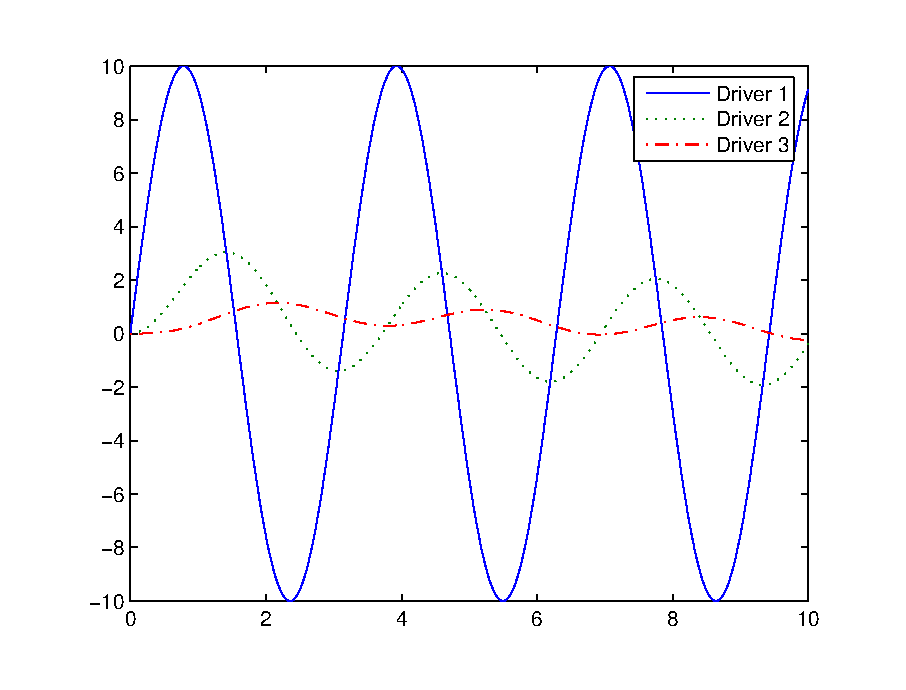
\includegraphics[width=\textwidth]{traffic_flow_3cars_ODE_l04}
\end{center}
$\lambda=0.4$
}
\frame{
\begin{center}
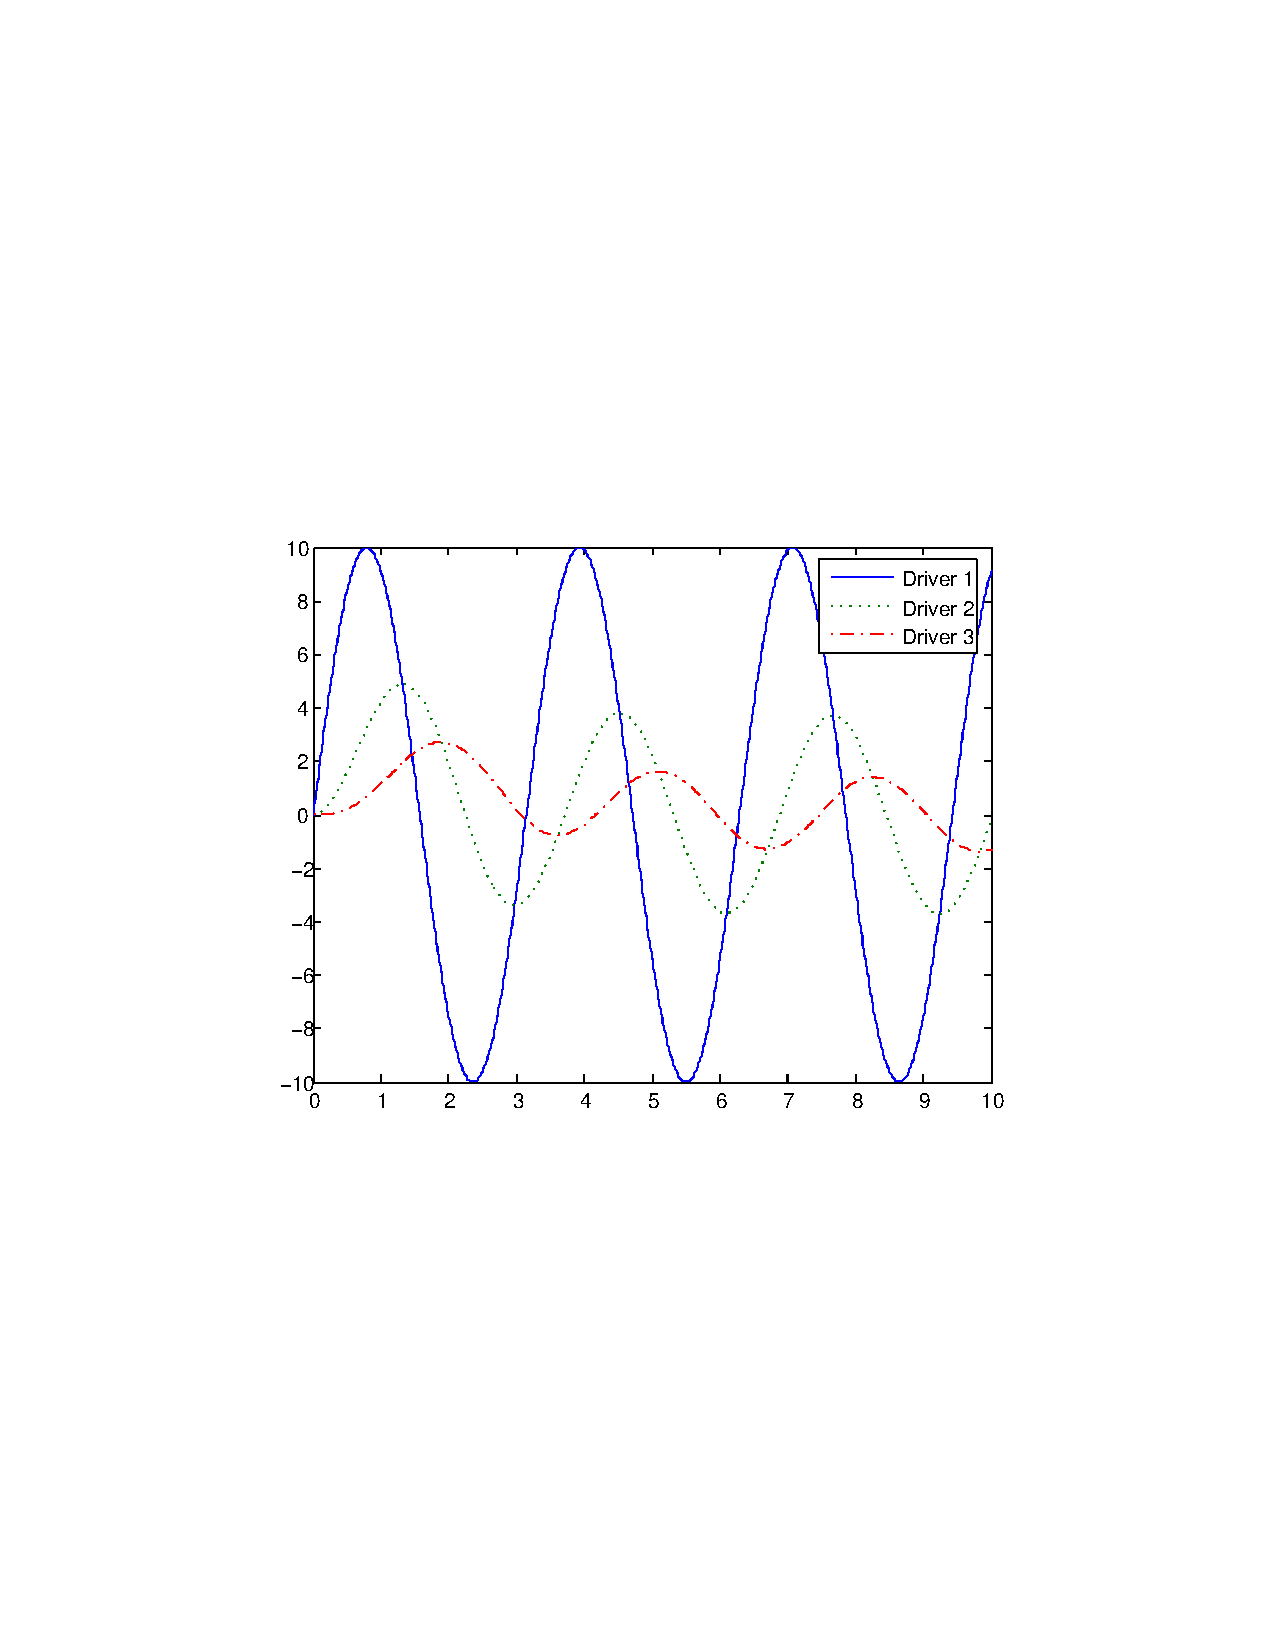
\includegraphics[width=\textwidth]{traffic_flow_3cars_ODE_l08}
\end{center}
$\lambda=0.8$
}
\frame{
\begin{center}
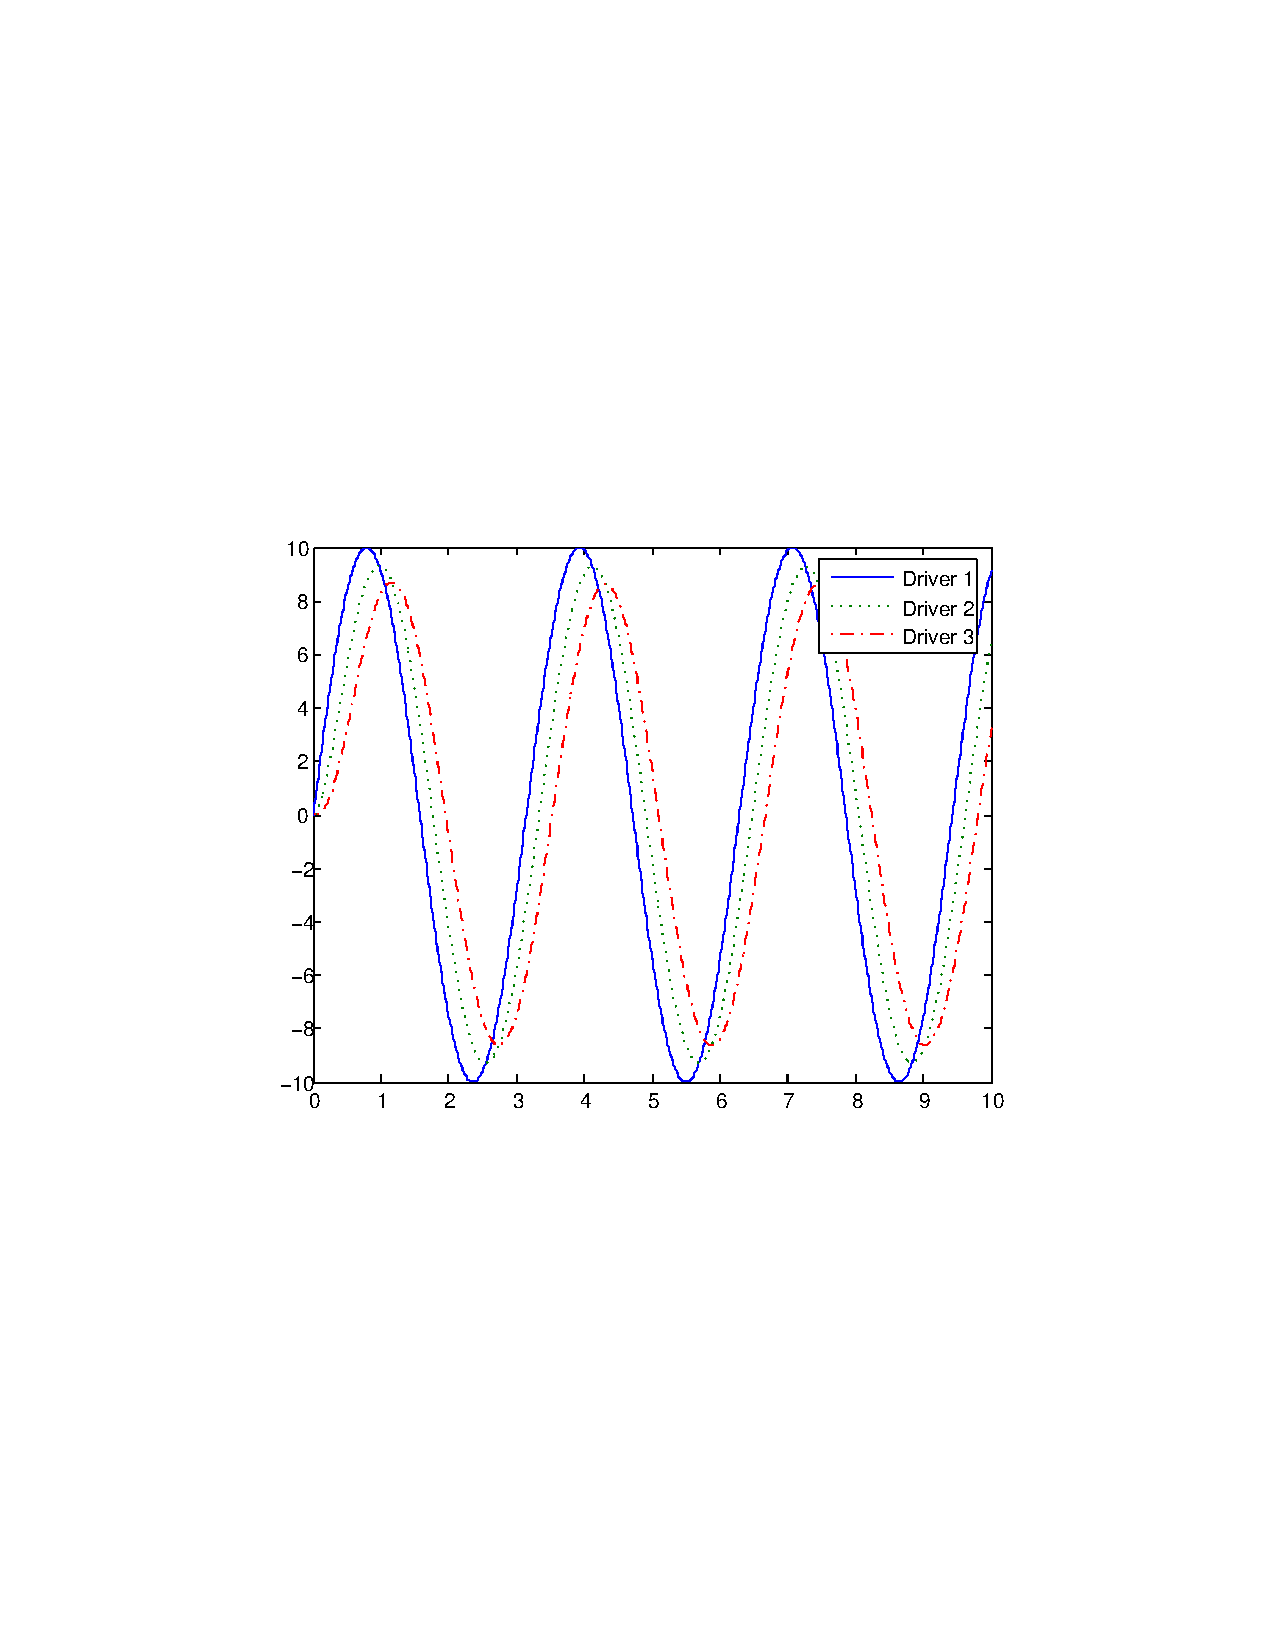
\includegraphics[width=\textwidth]{traffic_flow_3cars_ODE_l5}
\end{center}
$\lambda=5$
}


\section{Traffic flow -- DDE model}
\frame[plain]{\tableofcontents[current]}


\frame{\frametitle{A delay differential equations model}
\begin{itemize}
\item
In the previous model, reaction time is instantaneous.
\item
In practice, this is known to be incorrect: reflexes and psychology play a role.
\item
It takes at least a few instants to acknowledge a change of speed in the car in front.
\item
If the change of speed is not threatening, then you may not want to react right away.
\item 
When you press the accelerator or the brake, there is a delay between the action and the reaction..
\end{itemize}
}

\frame{\frametitle{A delayed model of traffic flow}
We consider the same setting as previously, except that now, for $t>0$,
\begin{equation}\label{eq:dde}
u'_{n+1}(t)=\lambda(u_n(t-\tau)-u_{n+1}(t-\tau)),
\end{equation}
for $n=1,\ldots,N-1$. Here, $\tau\geq 0$ is called the \emph{time delay} (or \emph{time lag}), or for short, \emph{delay} (or \emph{lag}).

\vskip1cm
If $\tau=0$, we are back to the previous model.
}

\frame{\frametitle{Initial data}
For a delay equation such as \eqref{eq:dde}, the initial conditions become \emph{initial data}. This initial data must be specified on an interval of length $\tau$, left of zero.
\vskip0.5cm
This is easy to see by looking at the terms: $u(t-\tau)$ involves, at time $t$, the state of $u$ at time $t-\tau$. So if $t<\tau$, we need to know what happened for $t\in[-\tau,0]$.
\vskip0.5cm
So, normally, we specify initial data as
\[
u_n(t)=\phi(t)\textrm{ for }t\in[-\tau,0],
\]
where $\phi$ is some function, that we assume to be continuous. We assume $u_1(t)$ is known.
\vskip0.5cm
Here, we assume, for $n=1,\ldots,N$,
\[
u_n(t)=0,\qquad t\leq (n-1)\tau
\]
}

\frame{\frametitle{Important remark}
Although \eqref{eq:dde} looks very similar to \eqref{eq:ode}, you must keep in mind that it is in fact much more complicated.
\begin{itemize}
\item
A solution to \eqref{eq:ode} is a continuous function from $\IR$ to $\IR$ (or to $\IR^n$ if we consider the system).
\item
A solution to \eqref{eq:dde} is a continuous function in the space of continuous functions.
\item
The space $\IR^n$ has dimension $n$. The space of continuous functions has dimension $\infty$.
\end{itemize}
We can use the Laplace transform to get some understanding of the nature of the solutions.
}

\section{The Laplace transform}
\frame[plain]{\tableofcontents[current]}

\frame{\frametitle{The Laplace transform}
\begin{definition}[Laplace transform]
Let $f(t)$ be a function defined for $t\geq 0$. The \emph{Laplace transform} of $f$ is the function $F(s)$ defined by
\[
F(s)=\L\{f(t)\}=\int_0^\infty e^{-st}f(t)dt.
\]
\end{definition}
The Laplace transform is a linear operator:
\[
\L\{af(t)+bg(t)\}=a\L\{f(t)\}+b\L\{g(t)\}.
\]
}

\frame{\frametitle{Rules of transformation}
\begin{center}
\begin{tabular}{ll}
$t$-domain & $s$-domain\\
\hline
$af(t)+bg(t)$ & $aF(s)+bG(s)$ \\
$tf(t)$ & $-F'(s)$ \\
$t^nf(t)$ & $(-1)^nF^{(n)}(s)$ \\
$f'$ & $sF(s)-f(0)$ \\
$f''$ & $s^2F(s)-sf(0)-f'(0)$ \\
$f^{(n)}$ & $s^nF(s)-s^{n-1}f(0)-\cdots-f^{(n-1)}(0)$ \\
$\frac{f(t)}{t}$ & $\int_s^\infty F(u)du$ \\
$\int_0^t f(u)du=u(t)\ast f(t)$ & $\frac 1s F(s)$ \\
$f(at)$ & $\frac 1{|a|}F\left(\frac sa\right)$ \\
$e^{at}f(t)$ & $F(s-a)$ \\
$f(t-a)u(t-a)$ & $e^{-as}F(s)$ \\
$f(t)\ast g(t)$ & $F(s)G(s)$
\end{tabular}
\end{center}
Here $f^{(n)}$ represents the $n$th derivative, not the $n$th iterate. $\ast$ is the convolution product.
}

\frame{\frametitle{Dirac delta -- Heaviside function}
In the table on the following slide,
\begin{itemize}
\item $\delta(t)$ is the Dirac delta,
\[
\delta(t)=\begin{cases}
\infty & \textrm{if }t=0\\
0 & \textrm{if }t\neq 0.
\end{cases}
\]
\item $H(t)$ is the Heaviside function,
\[
H(t)=\begin{cases}
0 & \textrm{if }t< 0 \\
1 & \textrm{if }t> 0
\end{cases}
\]
\end{itemize}
Note that $H(t)=\int_{-\infty}^t \delta(s)ds$.
}

\frame{\frametitle{Transforms of common functions}
\begin{center}
\begin{tabular}{ll}
$t$-domain & $s$-domain\\
\hline
$\delta(t)$ & $1$ \\
$\delta(t-\tau)$ & $e^{-\tau s}$ \\
$H(t)$ & $\frac 1s$ \\
$H(t-\tau)$ & $\frac{e^{-\tau s}}s$ \\
$\frac{t^n}{n!}H(t)$ & $\frac{1}{s^{n+1}}$ \\
$e^{-\alpha t}H(t)$ & $\frac 1{s+\alpha}$ \\
$\sin(\omega t)H(t)$ & $\frac{\omega}{s^2+\omega^2}$ \\
$\cos(\omega t)H(t)$ & $\frac s{s^2+\omega^2}$ \\
\end{tabular}
\end{center}
}

\frame{\frametitle{Inverse Laplace transform}
\begin{definition}
Given a function $F(s)$, if there exists $f(t)$, continuous on $[0,\infty)$ and such that
\[
\L\{f\}=F,
\]
then $f(t)$ is the \emph{inverse Laplace transform} of $F(s)$, and is denoted $f=\L^{-1}\{F\}$.
\end{definition}
\begin{theorem}
The inverse Laplace transform is a linear operator. Assume that $\L^{-1}\{F_1\}$ and $\L^{-1}\{F_2\}$ exist, then
\[
\L^{-1}\{aF_1+bF_2\}=a\L^{-1}\{F_1\}+b\L^{-1}\{F_2\}.
\]
\end{theorem}
}

\frame{\frametitle{Solving differential equations using the Laplace transform}
\begin{enumerate}
\item Take the Laplace transform of both sides of the equation.
\item Using the initial conditions, deduce an algebraic system of equations in $s$-space.
\item Solve the algebraic system in $s$-space.
\item Take the inverse Laplace transform of the solution in $s$-space, to obtain the solution of the differential equation in $t$-space.
\end{enumerate}
}

\section[Laplace of the DDE]{Laplace transform of our DDE traffic flow model}
\frame[plain]{\tableofcontents[current]}

\frame{
Let
\[
U_{k+1}(s)=\L\{u_{k+1}(t)\}=\int_0^\infty e^{-st}u_{k+1}(t)dt.
\]
Since we have assumed initial data of the form
\[
u_n(t)=0\qquad\textrm{for } t\leq(n-1)\tau,
\]
we have
\[
U_{k+1}(s)=\int_{k\tau}^\infty e^{-st}u_{k+1}(t)ds.
\]
}

\frame{
Since $u_{n+1}(t)=0$ for $t\leq n\tau$,
\begin{align*}
\int_0^\infty e^{-st}u_{n+1}'(t)dt &= \left[u_{k+1}(t)e^{-st}\right]_{k\tau}^\infty +s\int_{k\tau}^\infty e^{-st}u_{k+1}(t)dt \\
&= sU_{k+1}(s)
\end{align*}
and
\begin{align*}
\int_0^\infty e^{-st}u_{k+1}(t-\tau)dt &= \int_{(k-1)\tau}^\infty e^{-st}u_{k+1}(t-\tau)dt \\
&= \int_{(k-2)\tau}^\infty e^{-s(t+\tau)}u_k(\tau)d\tau \\
&= e^{-s\tau}U_k(s),
\end{align*}
since $e^{-st}u_{k+1}(t)\to 0$ for the improper integral to exist.

Note that we could have obtained this directly using the properties of the Laplace transform.
}

\frame{
Multiply 
\[
u_{n+1}'(t)=\lambda(u_{n}(t-\tau)-u_{n+1}(t-\tau))
\]
by $e^{-st}$,
\[
e^{-st}u_{n+1}'(t)=\lambda e^{-st}(u_{n}(t-\tau)-u_{n+1}(t-\tau))
\]
integrate over $(0,\infty)$ (using the expressions found above),
\[
sU_{n+1}(s)=\lambda(e^{-s\tau}U_{n}(s)-e^{-s\tau}U_{n+1}(s))
\]
which is equivalent to
\[
U_{n+1}(s)=\frac{\lambda U_n(s)}{\lambda+se^{s\tau}}
\]
Thus, when $U_1(s)$ is known, we can deduce the values for all $U_n$.
}

\frame{
Suppose 
\[
u_1(t)=\alpha \sin(\omega t)
\]
From the table of Laplace transforms, it follows that 
\[
U_1(s)=\alpha\frac{\omega}{s^2+\omega^2}
\]
Therefore,
\[
U_2=\frac{\lambda U_1(s)}{\lambda+se^{st}}
=\alpha\frac{\lambda}{\lambda+se^{st}}\;\frac{\omega}{s^2+\omega^2}
\]
and we can continue.. 
\vskip0.5cm
However, even though we know the solution in $s$-space, it is difficult to get the behavior in $t$-space, by hand, and maple does not help us either.
}


\end{document}